\documentclass[conference]{IEEEtran}
\IEEEoverridecommandlockouts
% The preceding line is only needed to identify funding in the first footnote. If that is unneeded, please comment it out.
\usepackage{cite}
\usepackage{amsmath,amssymb,amsfonts}
\usepackage{algorithmic}
\usepackage{graphicx}
\usepackage{hyperref}
\usepackage{subcaption}
\usepackage{textcomp}
\usepackage{xcolor}
\def\BibTeX{{\rm B\kern-.05em{\sc i\kern-.025em b}\kern-.08em
    T\kern-.1667em\lower.7ex\hbox{E}\kern-.125emX}}

\hypersetup{
    colorlinks=true,
    linkcolor=blue,
    filecolor=magenta,
    urlcolor=cyan,
}

\begin{document}

\title{FaceNet Clustering Analysis}

\author{
\IEEEauthorblockN{Rodrigo Castiel}
\IEEEauthorblockA{\textit{Center for Informatics} \\
\textit{Federal University of Pernambuco}\\
Recife, Brazil \\
rcrs2@cin.ufpe.br}
}


\maketitle

\begin{abstract}
In the last decade, deep-learning based techniques brought us a remarkable breakthrough in face recognition.
Recently, Google Researchers proposed \textit{FaceNet}, a novel face recognition system that learns a mapping from face pictures to a feature-space where similarities are well described by simple euclidean distances \cite{??}.
FaceNet may be combined with different clustering methods and classifiers; on famous face recognition databases, it currently achieves the best accuracy.
In this paper, we use FaceNet as a feature extractor to perform a face clustering analysis on three different databases: a small personal dataset, Labeled Faces in the Wild (LFW) and MUCT.
Our goal is to group pictures by person.
We run k-means, agglomerative clustering, spectral clustering, DBSCAN and mean-shift with different parameters on all datasets.
Experiments show that both DBSCAN and mean-shift achieve the best adjusted rand scores without even requiring the number of clusters in advance.

\end{abstract}

\begin{IEEEkeywords}
clustering, deep-learning, face recognition, facenet
\end{IEEEkeywords}

\section{Introduction}

\section{Clustering Analysis}

\subsection{Databases}

In this project, we chose three face databases with different properties to evaluate the quality of the clustering methods.
The first database, \textit{personal\_faces}, is a toy dataset of pictures of our teammates and classmates under random lighting and environmental conditions.
The second database is \textit{Labeled Faces in the Wild} (LFW) \cite{??}, a large database of famous people under random circumstances.
The third database is \textit{MUCT} \cite{??}, a reasonably large dataset of people under multiple predetermined lighting and camera angles.
Both \textit{personal\_faces} and LFW contain an uneven number of face pictures per person, while MUCT has the same picture styles for every person.
We picked \textit{personal\_faces} to perform a semantics analysis of the error pictures in a simple and clear way.

Given the raw database, we use OpenCV's cascade classifier to detect faces in the pictures \cite{??}.
It does not always find valid faces in an image, which makes the number of extracted faces to be slightly lower than the actual dataset size.
\textit{personal\_faces} contains $N = 59$ face pictures distributed over $K = 18$ clusters (people).
MUCT contains $N = 3710$ faces distributed over $K = 276$ clusters.
LFW originally contains $N = 13233$ faces distributed over $K = 5749$ people, but we filter out clusters with less than three pictures.
Therefore, the processed LFW database contains $N = 7400$ faces from $K = 901$ people.

Figure \ref{tsneview} (a) is a visualization of the \textit{personal\_faces} dataset in feature-space.
Notice that clusters are located in disjoint regions with clear boundaries.
Figure \ref{tsneview} (b) shows the clusters in LFW.
Due to its large volume, its several different ethnical groups and picture angles, it presents multiple overlaps between clusters.
The size and the scattering of its clusters are uneven.
Figure \ref{tsneview} (c) depicts MUCT.
There is much less overlapping than in LFW; in general, clusters are dense and clearly separable.

\begin{figure}[h]
  \begin{subfigure}[b]{0.5\textwidth}
    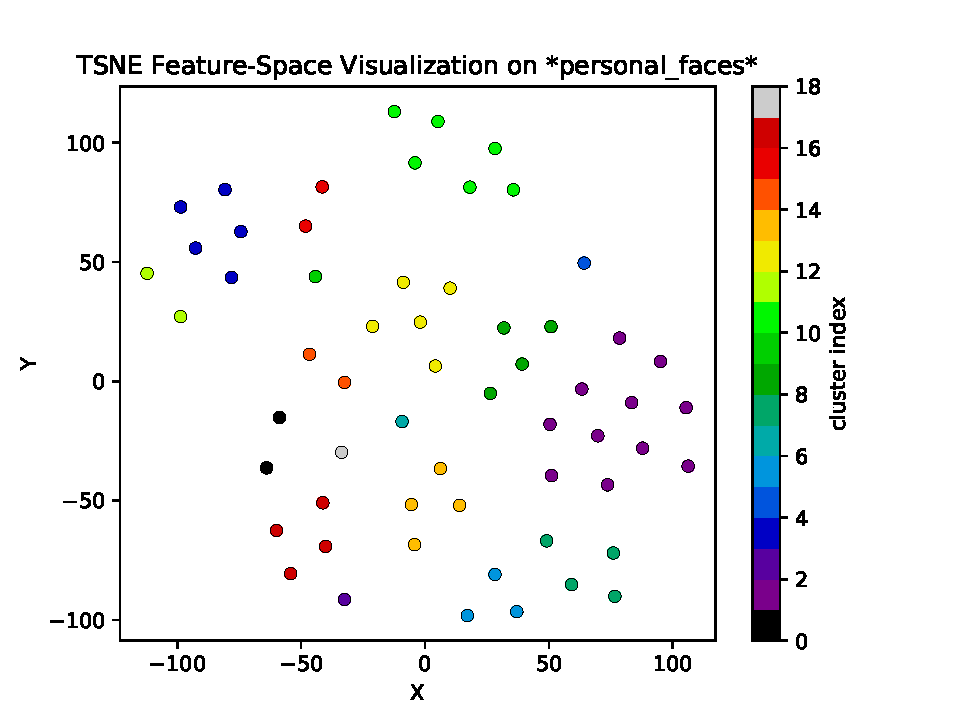
\includegraphics[width=\linewidth]{tsne_view_personal_faces}
    \caption{}
  \end{subfigure}
  \begin{subfigure}[b]{0.5\textwidth}
    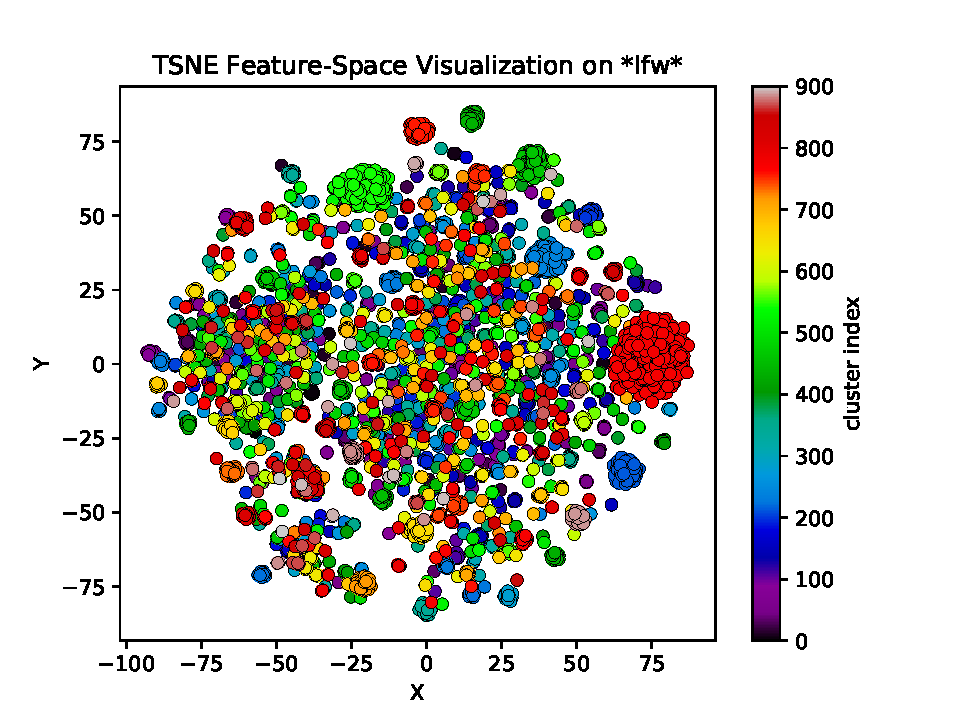
\includegraphics[width=\linewidth]{tsne_view_lfw}
    \caption{}
  \end{subfigure}
  \begin{subfigure}[b]{0.5\textwidth}
    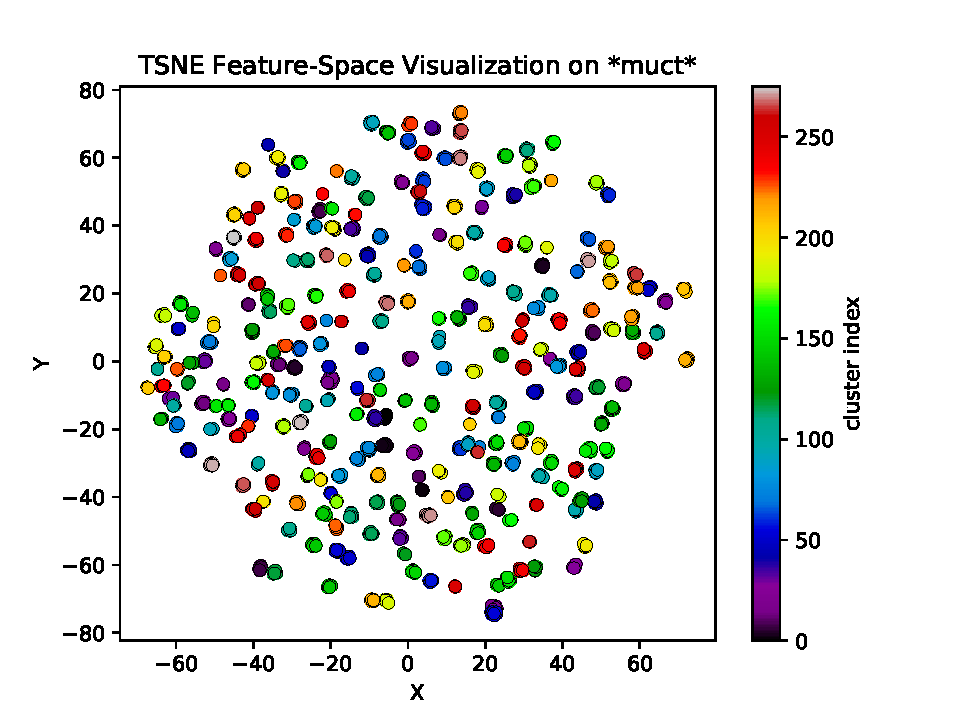
\includegraphics[width=\linewidth]{tsne_view_muct}
    \caption{}
  \end{subfigure}
  \caption{TSNE visualization of multiple databases in a 2D feature-space. Cluster indices are assigned to random colors. (a) personal\_faces. (b) LFW. (c) MUCT.}
  \label{tsneview}
\end{figure}

\subsection{Experiments}

\begin{figure}[h]
  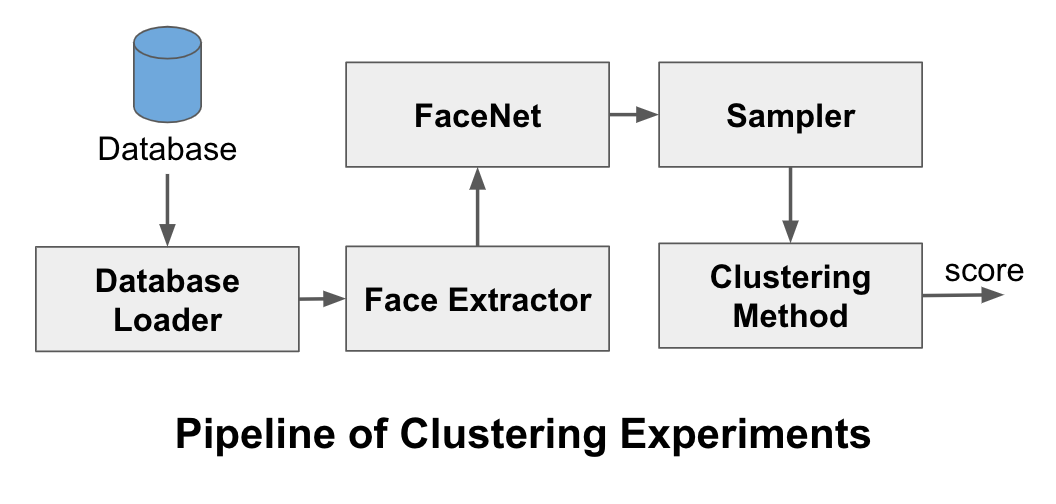
\includegraphics[width=\linewidth]{pipeline.png}
  \caption{Validation set creation pipeline.}
  \label{pipeline}
\end{figure}

In order to properly assess the quality of the clustering techniques, we evaluate the \textit{adjusted rand index} (or simply $ARI$ \cite{??}) of each method on a series of random subsets sampled from the entire input databases.
Each clustering method, with its given parameter values, is executed $n_{eval} = 30$ times on a randomly sampled subset whose size is approximately $80\%$ of the database size.
At the end, we compute the average $ARI$ score of each set of runs.
Figure \ref{pipeline} depicts the stages of our clustering experiments.

Recall that k-means, agglomerative clustering and spectral clustering need a hyper-parameter $K$, that is, the number of clusters to be found.
If $K$ is less than the actual number of people, these methods will tend to group similar people into the same clusters.
For example, pictures of people who share the same ethnical group, or who grow beard.
Though we could exhaustively tweak $K$ until we find the best $ARI$ score, we will not have a reference in practice, since no ground-truth labels are provided.
Therefore, for comparison purposes, we assume that $K$ is known.
Thus, this will give us a good upperbound for their scores.

On the other hand, we run mean-shift and DBSCAN with different hyper-parameter values.
As described in the following section, experiments suggest that both of them are roughly invariant to the real number of clusters.
In other words, their best hyper-parameters are about the same for any database.

\subsection{Results}

\subsubsection{Score Analysis}

Add table of all average scores (method vs. dataset).

Briefly explain table results.

Explain why DBSCAN and mean-shift are the best options.

\subsubsection{DBSCAN and Mean-shift parameter analysis}

Add plot of score vs eps and score vs bandwidth.

Explain plots.

\subsubsection{Semantics Analysis}

Explain secondary tool that groups photos.

Write about problems with sunglasses, ethnical groups, etc.

Write that agglomerative clustering finds the best grouping when K is known.

\section{Conclusion}

Write about the advantages of DBSCAN and mean-shift.

Write about downsides of facenet (sunglasses, for example).
Explain why classification can be better than clustering.

\begin{thebibliography}{00}
\bibitem{b1} Francisco de A.T. de Carvalho, Eduardo C. Simões, Lucas V.C. Santana, Marcelo R.P. Ferreira,
Gaussian kernel c-means hard clustering algorithms with automated computation of the width hyper-parameters,
Pattern Recognition,
Volume 79,
2018,
Pages 370-386,
ISSN 0031-3203,
https://doi.org/10.1016/j.patcog.2018.02.018.

\bibitem{b2} Vision Group, University of Massachusetts, 
Image Segmentation Data,
http://archive.ics.uci.edu/ml/machine-learning-databases/image/.

\end{thebibliography}

\end{document}
